\chapter{\label{ch:6-eval}Evaluation}

\minitoc

In this chapter, we evaluate our proposed approach. We start by describing a method for randomly generating benchmark FMU dependency graphs. Then, we present the obtained results. Finally, we give the speedup and accuracy results obtained by applying our approach on an industrial use case.

\section{Random Generator of Dependence Graphs}

Due to the difficulty in acquiring enough industrial FMU co-simulation applications for assessing our approach, we had to use a random generator of FMU dependence graphs. The generator creates the graphs and characterizes them with attributes.

\subsection{Random Dependence Graph Generation}

The random generator that we have implemented is inspired by the work of [Kalla:04]. However it differs from this work because the generation is done in two stages. In fact, we have to generate, first, the different FMUs of the co-simulation and their internal structures. Second, we generate the dependence graph by creating inter-FMU dependencies in such a way that the resulting operation graph is a DAG. Our generator is based on a technique of assignment of operations to levels. The dependence graph can then be visualized on a grid of levels as depicted in figure \ref{}. The generator uses of the following parameters:
\begin{itemize}
\item The graph size $n$: The number of operations;
\item The number of FMUs $m$;
\item The graph height $h$: The number of levels in the graph
\item The graph width $w$: The maximum number of nodes on one level
\end{itemize}
Note that parameters $n$ and $m$ are related. In other words, for a given size of a graph $n$, an adequate number of FMUs $m$ has to be chosen. The generation of the dependence graph is performed as follows:
\begin{itemize}
\item \textbf{Input:} Size of the graph $n$, number of FMUs $m$, height of the graph $h$, and width of the graph $w$. The number of FMUs can be derived automatically from the size of the graph using a predefined formula. For instance, one of the formulas that we have used is $ m = 5 \times log10(n/5)$. This allows to have adequate size of the graph and number of FMUs. Suppose for example that we have a size $n = 1000$ and a number of FMUs $m = 1$. Obviously, this example does not represent a realistic application. 
\item \textbf{Step 1:} Randomly distribute the $n$ operations to the $m$ FMUs. Given the number of operations of each FMU, we randomly determine the number of its input operations and the number of its output operations. Every operation has one state operation.
\item \textbf{Step 2:} Randomly generate the intra-FMU arcs. This step is controlled by two parameters.  The number of arcs to generate and the number of NDF outputs of the FMU. These outputs are not considered when randomly generating the arcs.
\item \textbf{Step 3:} Randomly assign the operations to the grid levels. This step is performed by assigning output operations and then input operations repeatedly.
\begin{enumerate}
\item Assign all NDF operations to level $0$ of the grid.
\item Randomly assign remaining output operations to even levels $lvl \in {2, 4, \ldots, h-3} $ of the grid.
\item Assign the input operations to the odd levels $lvl \in {1, 3, \ldots, h-4} $ of the grid such that any input operation $o_i$ that is connected to an output operations $o_j$ (intra-FMU dependence) is assigned to the level preceding the level to which $o_j$ has been assigned. 
\item Assign the remaining input operations (each of which is not connected with any output operation) to the level $h-2$ of the grid. These operations will be connected only with the state operations of their respective FMUs.
\item Add the state operations to the last level of the grid.
\end{enumerate}
\item \textbf{Step 4:} Create the arcs of the dependence graph. At this step we randomly generate inter-FMU dependencies. For each operation $o_i$ on the level $lvl$ of grid, we randomly select an output operation $o_j$ from the preceding level $lvl-1$ and which belongs to a different FMU than $o_i$. We create an arc from $o_j$ to $o_i$. If no such output operation is found at level $lvl-1$, we select randomly an output operation from any level $lvl' < lvl-1$ and connect it with the operation $o_i$. Finally the arcs from input and output operations to state operations are created. 
\end{itemize}

\subsection{Random Dependence Graph Characterization}

In addition to random generation of the dependence graph structure, we need to generate the attributes of the graph. In particular, the following attributes are generated by our random generator:
\begin{itemize}
\item Communication steps of the FMUs.
\item Execution times of the operations. The execution times are generated randomly in such a way that state operations have longer execution times than the output and input operations
\end{itemize}

\section{Results}

\section{Industrial Use Case}

The proposed parallelization approach has been applied on an industrial use case. In this section, we give a description of the use case and then present the obtained results. 

Tests have been performed on a computer running the Windows 7 operating system with 16 GB RAM and an Intel core i7 processor running 8 cores at 2.7 GH. Experiments have been carried out on a Spark Ignition (SI) RENAULT F4RT engine co-simulation. It is a four-cylinder in line Port Fuel Injector (PFI) engine in which the engine displacement is 2000 $cm^3$. The air path is composed of a turbocharger with a mono-scroll turbine controlled by a waste-gate, an intake throttle and a downstream-compressor heat exchanger. This co-simulation is composed of 5 FMUs: one FMU for each cylinder and one FMU for the airpath. The FMUs were imported into xMOD using the FMI export features of the Dymola tool. This use-case leads to an initial graph containing over 100 operations. We refer to our proposed method as MUO-RCOSIM (for Multi-Rate Oriented RCOSIM). We compared the obtained results with two approaches: The first one is RCOSIM which is mono-rate and thus we had to use the same communication step for all the FMUs. We used a communication step of $20 {\mu}s$. The second one consists in using RCOSIM with the multi-rate graph transformation algorithm. We refer to it as MU-RCOSIM (for Multi-Rate RCOSIM). For MUO-RCOSIM and MU-RCOSIM we used the recommended configuration of the communication steps for this use case. For each cylinder, we used a communication step of $20 {\mu}s$. The communication step used for the airpath is $100 {\mu}s$. In fact, the airpath has slower dynamics than the cylinders and this configuration of the communication steps corresponds to the specification given by engine engineers. For each FMU, we used a Runge-Kutta 4 solver with a fixed integration step equal to the communication step. The graph of this use case is transformed by Algorithm \ref{algo:mr} into a graph containing over 280 operations that are scheduled by the multi-core scheduling heuristic.      

The validation of the numerical results of the co-simulation using the proposed method is achieved through the comparison of the co-simulation outputs with reference outputs. Since it is not possible to solve the equations of the FMU analytically, the reference outputs are obtained by using RCOSIM which has been shown in \cite{benkhaled:2014} to give a very good accuracy of the numerical results. Figure \ref{fig:df} shows the obtained results for the torque (an output of the airpath). We note that the results match with the reference, and the generated error is very small remaining within an acceptable bound ($< 1\%$). Similar accuracy results were obtained for the different outputs of the co-simulation.

The speedup obtained using MUO-RCOSIM is compared with the speedups obtained using RCOSIM and MU-RCOSIM. The speedup was evaluated by running the co-simulation in xMOD. Execution times measurements were performed by getting the system time stamp at the beginning and at the end of the co-simulation. For a given run of the co-simulation, the speedup is computed by dividing the mono-core co-simulation execution time of RCOSIM by the co-simulation execution time of this run on a fixed number of cores. Figure \ref{fig:spdup} sums up the results. The same speedup is obtained using MUO-RCOSIM and MU-RCOSIM even when only 1 core is used. This speedup is obtained thanks to using the multi-rate configuration. More specifically, increasing the communication step of the airpath from $20 {\mu}s$ to $100 {\mu}s$ results in fewer calls to the solver leading to an acceleration in the execution of the co-simulation. By using multiple cores, speedups are obtained using both MUO-RCOSIM and MU-RCOSIM. Additionally, MUO-RCOSIM outperforms MU-RCOSIM with an improvement in the speedup of, approximately $30\%$ when 2 cores are used, and approximately $10\%$ when 4 cores are used. This improvement is obtained thanks to the acyclic orientation heuristic which defines an efficient order of execution for the operations of each FMU that are mutually exclusive. This defined order tends to allow the multi-core scheduling heuristic to better adapt the potential parallelism of the operation graph to the effective parallelism of the multi-core processor (number of cores) resulting in an improvement in the performance. MU-RCOSIM, on the other hand, uses the solution of RCOSIM which consists in simply allocating mutual exclusive operations to the same core introducing restrictions on the possible solutions of the multi-core scheduling heuristic. When using 8 cores, no further improvement is possible since the potential parallelism is fully exploited. Worse still, the overhead of the synchronization between the cores becomes counter-productive, which explains why the speedup with 8 cores is less than the speedup with 4 cores for all the approaches. The best performance is obtained using 5 cores with slight improvement compared to using 4 cores. 

\begin{figure}[htb]
\centering
  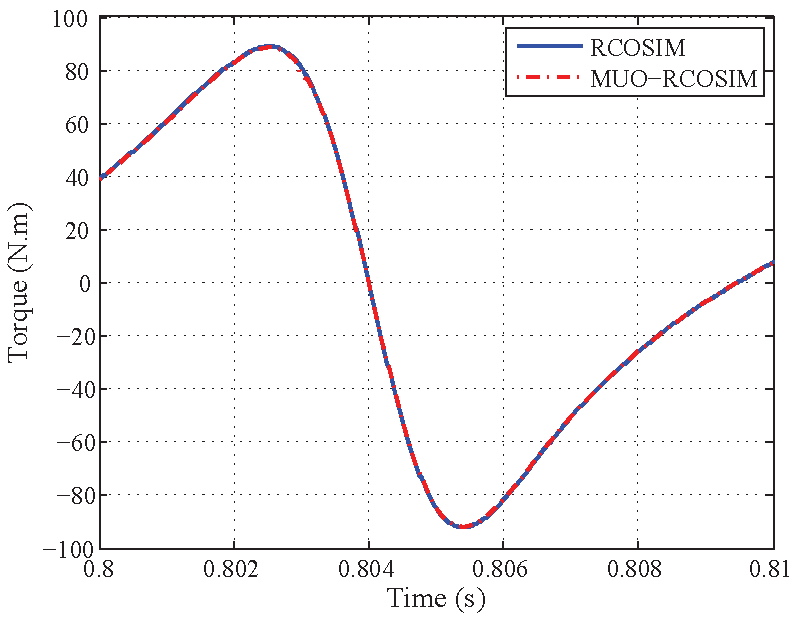
\includegraphics[scale=0.8]{figures/DF}
  \caption{Numerical results}
  \label{fig:df}
\end{figure}

\begin{figure}[htb]
\centering
  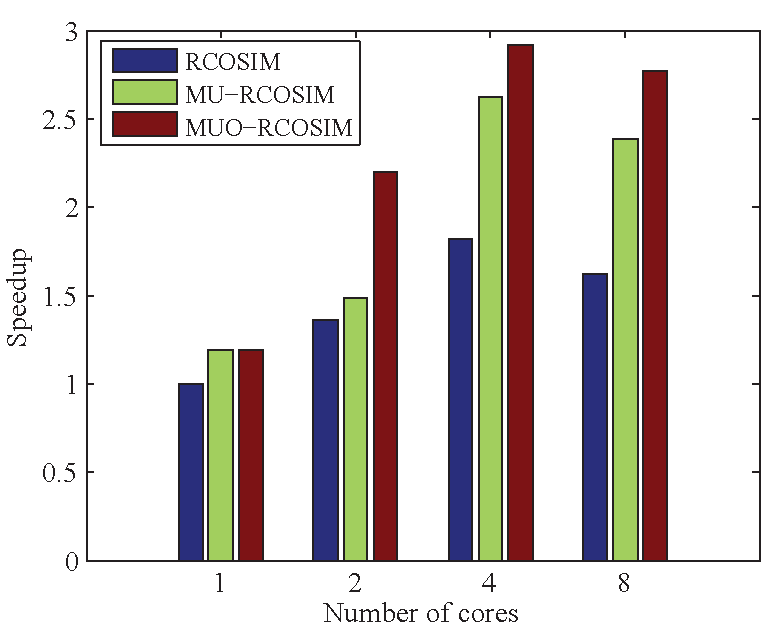
\includegraphics[scale=0.8]{figures/Speedup}
  \caption{Speedup results}
  \label{fig:spdup}
\end{figure}  

The obtained speedup and numerical accuracy results show the efficiency of our proposed method. In future work, we aim at comparing our solution with an exact scheduling algorithm and also an online scheduling approach. Also, we will test our proposed method on other industrial applications. In addition, we envision to extend MUO-RCOSIM to real-time multi-core scheduling in order to perform Hardware-in-the-Loop simulation whose main challenge is to map the real-time constraints on the different operations of the graph.